
In order to allow different scheduling strategies, we introduce the concept of
\emph{node priority} by assigning a priority value to every node in the program
and by introducing coordination facts that manipulate such priority values.  By
default, nodes have no priority and can be picked in any order. In our
implementation, we use a FIFO approach because older nodes tend to have a higher
number of unexamined facts, from which to derive subsequent new facts.

We have two kinds of priorities: a \emph{temporary priority} and a \emph{default
   priority}. A temporary priority momentarily changes the default priority $D$
of a node, so that once the node is done, the priority will default back to $D$.
Initially, all nodes have a default priority of $-\infty$.

The following list presents the action facts available to manipulate the
scheduling decisions of the system:

\begin{itemize}
   \item \code{set-priority(node A, float F)}: This sets the
   temporary priority of \texttt{A} to \texttt{F}. If \texttt{A} has priority
   \texttt{F'}, we only change the priority if \texttt{F} is higher. The programmer
   can decide if priorities are to be ordered in ascending or descending order.
   \item \code{add-priority(node A, float F)}: Increases,
   temporarily, the priority of node \texttt{A} by \texttt{F}.
   \item \code{remove-priority(node A)}: Removes the temporary priority from node
   \texttt{A}.
   \item \code{schedule-next(node A)}: Changes the temporary priority of node
   \texttt{A} to be $+\infty$.
   \item \code{set-default-priority(node, float)}: Sets the default
   priority of the node.
   \item \code{stop-program()}: Immediately stops the execution of the whole program.
\end{itemize}

LM provides the sensing fact \code{priority(node A, float P)} in order to sense
the priority \texttt{P} of node \texttt{A}. Sensing facts can only be used in
the body of rules and are exempt from the constraint that forces every fact used
in the body to have the same first argument. Also note that when sensing facts
are used to prove new facts, they are re-derived automatically. All the
coordination facts are linear and are consumed when used in the body of a rule.
The system creates the necessary code to re-derive them without programmer
interaction. Likewise, \texttt{set-priority} and \texttt{set-default-priority}
update the value of \texttt{priority} facts by retracting and re-asserting them
but this is done automatically by the runtime system.

The priorities assigned to nodes are respected on a thread basis, therefore a
thread will always pick the highest priority node on its sub-graph but not the
highest priority node of the whole graph.
Figure~\ref{fig:coordination:priorities} shows a graph that is being processed
by two threads \texttt{T0} and \texttt{T1}. The order for \texttt{T0} will be
\texttt{@0}, \texttt{1}, \texttt{@3}, \texttt{@2} and for thread \texttt{T1} it
will be \texttt{@4}, \texttt{@6}, \texttt{@5}.  Priorities can also be seen as
hints because they do not provide a global ordering but only a local ordering
that is somewhat similar to the global ordering. The only exception is
\texttt{schedule-next}, which, when the target node is located in the current
thread, will always be enforced.

Note that priorities of nodes can be set from any node in the graph, even if those nodes
live on different threads. Of course, this implies communication between
threads.

\begin{figure}
\begin{center}
   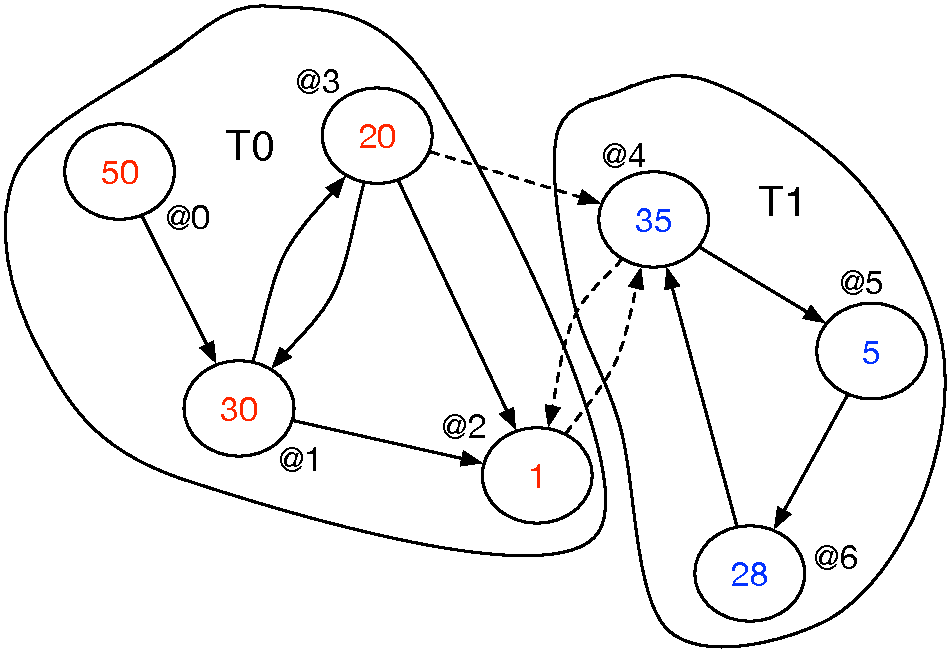
\includegraphics[width=0.7\textwidth]{figures/coordination/priorities.pdf}
\end{center}
\caption{Priorities with sub-graph partitioning. Priorities are used on a
   per-thread basis therefore thread \texttt{T0} schedules \texttt{@0} to
   execute, while \texttt{T1} schedules node \texttt{@4}.}
\label{fig:coordination:priorities}
\end{figure}
